% Generated with genpdf
% Domain Interno
% Title Piano di Qualifica
\documentclass{scalatekids-article}
\begin{document}
\lfoot{Piano Di Qualifica 1.0.0}
\newgeometry{top=3.5cm}
\begin{titlepage}
  \begin{center}
    \begin{center}
      
\includegraphics[width=10cm]{sklogo.png}
    \end{center}
    \vspace{1cm}
    \begin{Huge}
      \begin{center}
        \textbf{Piano di Qualifica}
      \end{center}
    \end{Huge}
    \vspace{11pt}
    \bgroup
    \def\arraystretch{1.3}
    \begin{tabular}{r|l}
      \multicolumn{2}{c}{\textbf{Informazioni sul documento}} \\
      \hline
      \setbox0=\hbox{0.0.1\unskip}\ifdim\wd0=0pt
      \\
      \else
      \textbf{Versione} & 0.0.3\\
      \fi
      \textbf{Redazione} & \multiLineCell[t]{Redattore}\\
      \textbf{Verifica} & \multiLineCell[t]{Verificatore}\\
      \textbf{Approvazione} & \multiLineCell[t]{Approvatore}\\
      \textbf{Uso} & Esterno\\
      \textbf{Lista di Distribuzione} & \multiLineCell[t]{ScalateKids\\Prof. Tullio Vardanega\\Prof. Riccardo Cardin}\\
    \end{tabular}
    \egroup
    \vspace{22pt}
  \end{center}
\end{titlepage}
\restoregeometry
\clearpage
\setcounter{page}{1}
\begin{flushleft}
  \vspace{0cm}
         {\large\bfseries Diario delle modifiche \par}
\end{flushleft}
\vspace{0cm}
\begin{center}
  \begin{tabular}{| l | l | l | l | l |}
    \hline
    Versione & Autore & Ruolo & Data & Descrizione \\
    \hline
    0.0.1 & Andrea Giacomo Baldan & & 2015-12-27 & Creazione scheletro del documento\\
    \hline
  \end{tabular}
\end{center}
\tableofcontents
\newpage
\section{Sommario}
\subsection{Scopo del documento}
Il seguente documento ha lo scopo di delineare le strategie che il gruppo \textit{ScalateKids} ha deciso di adottare per garantire degli obiettivi qualitativi da applicare ai processi sfruttati per lo sviluppo del progetto \textbf{ActorBase}. Per raggiungere tali obiettivi è necessario svolgere un'attività di verifica continua in modo da rilevare e correggere errori o malfunzionamenti minimizzando lo spreco di risorse.
\prodPurpose
\glossExpl
\subsection{Riferimenti}
\subsubsection{Normativi}
\begin{itemize}
\item\textbf{Capitolato d'appalto C1:} \textit{Actorbase: a NoSQL DB based on the Actor model;}\\
  \url{http://www.math.unipd.it/~tullio/IS-1/2015/Progetto/C1.pdf}
\item\textbf{Norme di Progetto:} \href{run:../Interni/NormeDiProgetto\_v1.0.0.pdf}{Norme di Progetto v1.0.0.}
\end{itemize}
\subsubsection{Informativi}
\begin{itemize}
\item\textbf{Piano di Progetto:} \href{run:./PianoDiProgetto\_v1.0.0.pdf}{Piano di Progetto v1.0.0}
\item\textbf{Dispense fornite dall'insegnamento Ingegneria del Software mod. A:}\\
  \url{http://www.math.unipd.it/~tullio/IS-1/2015/}
\item\textbf{Standard \gloss{ISO}/\gloss{IEC} 15504:}\\
\url{https://en.wikipedia.org/wiki/ISO/IEC_15504}
\item\textbf{Standard \gloss{ISO}/\gloss{IEC} 9126:}\\
\url{https://it.wikipedia.org/wiki/ISO/IEC_9126}
\item\textbf{\gloss{Ciclo di Deming}:}\\
\url{https://en.wikipedia.org/wiki/PDCA}
\end{itemize}
\newpage
\section{Visione generale della strategia di verifica}
\subsection{Definizione obiettivi}
\subsubsection{Qualità di processo}
Per perseguire la qualità del prodotto è necessario garantire la qualità dei processi attuati per la sua creazione. Per raggiungere questo scopo i \textit{Verificatori} con approvazione del \textit{Responsabile} hanno trovato utile adottare lo standard \gloss{ISO}/\gloss{IEC} 15504\footnote[1]{Per approfondimenti consultare la sezione \ref{sec:ISO/IEC15504}.} denominato SPICE (Software Process Improvement and Capability dEtermination). Il \gloss{ciclo di Deming}\footnote[2]{Per approfondimenti consultare la sezione \ref{PDCA}.} (noto anche come ciclo \gloss{PDCA}) è stato scelto per applicare correttamente questo standard. Esso definisce un metodo di controllo costante sui processi consentendo in questo modo un miglioramento incrementale della qualità continuo.
\subsubsection{Qualità di prodotto}
I \textit{Verificatori} con approvazione del \textit{Responsabile} hanno deciso di seguire lo standard \gloss{ISO}/\gloss{IEC} 9126\footnote[3]{Per approfondimenti consultare la sezione \ref{sec:ISO/IEC9126}.} che ha lo scopo di delineare delle metriche per la misurazione della qualità di prodotto. Questa è fondamentale per garantire che il prodotto \gloss{software} finale funzioni correttamente e rispetti degli obiettivi di qualità prefissati.
\subsection{Procedure di controllo di qualità di processo}
La qualità dei processi è assicurata dall'applicazione del ciclo \gloss{PDCA} a ogni processo. Tale metodo consente di migliorare continuamente ogni processo coinvolto nell’attività di sviluppo. Per applicare correttamente il ciclo \gloss{PDCA} è necessario avere una pianificazione di processi e risorse dettagliata. La descrizione dettagliata della pianificazione si trova nel \href{run:./PianoDiProgetto\_v1.0.0.pdf}{Piano di Progetto v1.0.0}.\\
\subsection{Procedure di controllo di qualità di prodotto}
Il controllo di qualità del prodotto si suddividerà in tre parti:
\begin{itemize}
\item{Attuazione di tecniche di analisi statica e dinamica descritte nella sezione \ref{sec:TecnicheDiAnalisi};}
\item{Verifica costante dell'output di ogni attività, i cui risultati verranno riportati nell'appendice \ref{sec:resAttivitaVerifica};}
\item{Validazione, ovvero la conferma che il prodotto risponda correttamente ai requisiti attesi.}
\end{itemize}
\subsection{Organizzazione}
Per garantire la qualità del prodotto finale verranno effettuate attività di verifica su ogni processo attuato. I controlli su ogni processo avranno come obiettivo garantire la qualità sia del processo stesso sia dell'eventuale prodotto da esso ricavato.\\
Ogni fase descritta in \href{run:./PianoDiProgetto\_v1.0.0.pdf}{Piano di Progetto v1.0.0} necessità di attività di verifica diverse a causa della differenza natura del loro output. Di seguito sono elencate le strategie di verifica usate per ciascuna fase:
\begin{itemize}
\item\textbf{Analisi:} durante questa fase verrà verificato che ogni documento creato sia conforme a quanto descritto nel documento \href{run:../Interni/NormeDiProgetto\_v1.0.0.pdf}{Norme di Progetto v1.0.0}, inoltre sarà necessario controllare che ogni requisito sia associato a un caso d'uso e viceversa;
\item\textbf{Progettazione:} durante questa fase l'attività di verifica si concentrerà sul processo incrementale dei documenti prodotti in fase di Analisi e sui processi attuati per l'attività di progettazione assicurandosi che ogni documento e ogni processo sia conforme a quanto descritto nelle \href{run:../Interni/NormeDiProgetto\_v1.0.0.pdf}{Norme di Progetto v1.0.0};
\item\textbf{Codifica:}durante questa fase l'attività di verifica si concentrerà sul processo incrementale dei documenti prodotti in fase di Analisi e sui processi attuati per l'attività di codifica assicurandosi che ogni documento e ogni processo sia conforme a quanto descritto nelle \href{run:../Interni/NormeDiProgetto\_v1.0.0.pdf}{Norme di Progetto v1.0.0}.
\end{itemize}
In ogni documento viene inoltre tenuto un diario delle modifiche per permettere di mantenere uno storico delle attività svolte su di esso e delle responsabilità per ogni attività.
\subsection{Pianificazione strategica e temporale}
L'attività di redazione di ogni documento sarà sempre anticipata da uno studio sulla struttura e sui contenuti del documento interessato. In questo modo si riduce la possibilità di errori concettuali e il tempo effettivo di scrittura del documento viene ridotto.\\
Il processo di verifica deve essere ben organizzato e pianificato per rispettare le scadenze fissate nel \href{run:./PianoDiProgetto\_v1.0.0.pdf}{Piano di Progetto v1.0.0}.\\
L'attività di verifica segue le metodologie descritte nelle \href{run:../Interni/NormeDiProgetto\_v1.0.0.pdf}{Norme di Progetto v1.0.0}. Esse sono state pensate in maniera tale da consentire l'individuazione e la correzione degli errori il più presto possibile evitando che si diffondano.
%TODO
\subsection{Responsabilità}
Per organizzare al meglio il lavoro e in particolare le \gloss{attività} di verifica e validazione vengono assegnati questi compiti ai soli \textit{Verificatori} e al \textit{Responsabile}. Inoltre le \gloss{attività} di verifica non potranno essere svolte da un membro che ha partecipato allo sviluppo di tale sezione per garantire assenza di conflitto di interessi (vedi norme.
\subsection{Tecniche di analisi}
\label{sec:TecnicheDiAnalisi}
\subsubsection{Analisi statica}
L'analisi statica è una tencica atta a trovare errori e anomalie. Questa tecnica è applicabile sia alla documentazione sia al codice.
\paragraph{Walkthrough}
\label{sec:walkthrough}Come descritto nelle \textit{\href{run:../Interni/NormeDiProgetto_v1.0.0.pdf}{Norme di Progetto v1.0.0}} verrà effettuata tecnica walkthrough nelle fasi iniziali di ogni \gloss{attività} per passare il prima possibile a \gloss{attività} di \textit{Inspection} (paragrafo seguente).
%TODO: linkiamo la lista di controllo?
\paragraph{Inspection}
\label{sec:inspection}Successivamente all'\gloss{attività} di \ref{sec:walkthrough}{Walthrough} verrà fatta \gloss{attività} di inspection (seguendo \textit{Norme di Progetto} (paragrafo precedente)) rispetto alla lista di controllo ottenuta in precedenza.
\subsubsection{Analisi dinamica}
L'analisi dinamica si applica solo al prodotto software e serve a trovare errori o difetti nell'implementazione.\\I test effettuati devono essere \textit{ripetibili}; questa caratteristica è fondamentale poichè un test deve produrre sempre lo stesso risultato dato un input in un ambiente per trovare errori.
\paragraph{Test di unità}
Test per verificare ogni unità del software prodotto. Per unità si intende la pià piccola quantità di software che è utile verificare singolarmente.\\L'obbliettivo di questi test è trovare ed eliminare possibili errori creati dai \textit{programmatori}.
\paragraph{Test di integrazione}
Test per verificare che l'integrazione tra due o più unità software funzionino correttamente.\\In mancanza di unità questi test possono essere svolti tramite la creazione di una o più componenti fittizie che simulano il comportamento delle unità con cui l'unità creata deve interfacciarsi. %TODO vabbe... mettere apposto sta frase
\paragraph{Test di sistema}
Test per verificare la totale copertura dei requisiti software emersi in fase di \textit{Analisi dei Requisiti}. Questi test verificano la totalità del prodotto software al suo raggiungimento di una versione definitiva.
\paragraph{Test di regressione}
Test da effettuare per verificare che una modifica del software non pregiudichi il funzionamento del sistema o di altre parti del prodotto prima correttamente funzionanti.\\
Questa attività dev'essere svolta tenendo conto del tracciamento dei requisiti per individuare i giusti test di unità, di integrazione e di sistema che possono essere influenzati dalle modifiche effettuate.\\
\paragraph{Test di accettazione}
Questo corrisponde al collaudo vero e proprio del software da svolgersi col \textit{Proponente}.

\subsection{Metriche di valutazione}
Per rendere quantificabile il processo di verifica verranno usate delle metriche elencate sotto. Soltando due tipi di \gloss{range} saranno accettati:
\begin{itemize}
  \item \textbf{Ottimale}: contiene i valori che si deve cercare di ottenere, valori al di fuori di questo range dovranno essere verificati e, se necessario, discussi dal gruppo;
  \item \textbf{Accettazione}: valori per avere un accetazione del prodotto.
\end{itemize}
\subsubsection{Metriche per i documenti}
Per la stesura dei documenti è stato scelto di utilizzare un \textit{indice di leggibilità} per la lingua italiana.
\paragraph{Indice Gulpease}
\label{par:metricheGulpease}
Questo indice indica il grado di leggibilità di un documento.\\L'indice di Gulpease prende in considerazione principalmente tre variabili:
\begin{itemize}
\item Numero delle frasi;
\item Numero delle lettere;
\item Numero delle parole.
\end{itemize}
La formula applicata per calcolare il suddetto indice è:
\begin{center}
\begin{equation}
  89 + \cfrac{300 * (numero delle frasi) - 10 * (numero delle lettere)}{numero delle parole}
\end{equation}
\end{center}
Lo script applicato su un documento produrrà in output un valore interno compreso tra zero e cento, in particolare i significati sono i seguenti:
\begin{itemize}
  \item Indice inferiore a 80 rappresenta un documento difficile da leggere per persone con una licenza di scuola elementare;
  \item Indice inferiore a 60 rappresenta un documento difficile da leggere per persone con una licenza di scuola media inferiore;
  \item Indice inferiore a 40 rappresenta un documento difficile da leggere per persone con una licenza di diploma superiore;
\end{itemize}
\textbf{Range accettabili:}
\begin{itemize}
  \item Range ottimale: 60 - 100;
  \item Range di accettazione: 45 - 60.
\end{itemize}
\subsubsection{Metriche per il software}
Per perseguire una buona qualità software sono state pensate diverse metriche di valutazione descritte nei prossimi paragrafi. Tuttavia questa sezione è una sezione che potrà subire cambiamenti durante le prossime revisioni.
\paragraph{Linee di codice per linee di commento}
Applicato su un file produrrà un valo0re in output che rappresenta la percentuale di righe di commento rispetto alle linee di codice.\\ 
\textbf{Range accettabili:}
\begin{itemize}
  \item Range ottimale: 30 - 40\%;
  \item Range di accettazione: 20 - 30\%.
\end{itemize}
\subsubsection{Copertura del codice}
La copertura del codice indica il numbero di istruzioni che vengono eseguite durante i test rispetto alla totalità delle istruzioni. Per avere una minor possibilità di presenza di errori nel codice si dovrà avere una percentuale il più alta possibile di istruzioni testate.\\Tuttavia metodi molto semplici che non necessitano testing andranno a influire negativamente in questo ambito.\\
\textbf{Range accettabili:}
\begin{itemize}
  \item Range ottimale: 60 - 100\%;
  \item Range di accettazione: 40 - 60\%.
\end{itemize}
\subsubsection{Numero di attributi per classe}
Un numero troppo elevato di attributi in una classe potrebbe indicare il non soddisfacimento del principio di \textit{\gloss{single responsability}}. Questo potrebbe significare la necessità di una divisione in più classi relazionate tra loro per dividere le diverse funzionalità o un possibile errore di progettazione.\\
\textbf{Range accettabili:}
\begin{itemize}
  \item Range ottimale: 3 - 6;
  \item Range di accettazione: 0 - 12.
\end{itemize}
\subsubsection{Numero di parametri per metodo}
Un numero troppo elevato di parametri in un metodo potrebbe indicare il non soddisfacimento del principio di \textit{\gloss{single responsability}}. Questo potrebbe significare la necessità di una divisione in sotto metodi per dividere le diverse funzionalità o un possibile errore di progettazione.\\
\textbf{Range accettabili:}
\begin{itemize}
  \item Range ottimale: 0 - 4;
  \item Range di accettazione: 4 - 8.
\end{itemize}
\subsubsection{Complessità ciclomatica}
La complessità ciclomatica è usata per misurare la complessità di parti di codice come funzioni, metodi, classi o moduli.\\
Questa è calcolata attraverso un grafo di controllo del flusso del programma.\\La complessità ciclomatica di una sezione di codice è il numero di cammini linearmente indipendenti attraverso il codice sorgente. Per esempio, se il codice sorgente non contiene punti decisionali come IF o cicli FOR, allora la complessità sarà 1, poiché esiste un solo cammino nel sorgente (e quindi nel grafo). Se il codice ha un singolo IF contenente una singola condizione, allora ci saranno due cammini possibili: il primo se l'IF viene valutato a TRUE e un secondo se l'IF viene valutato a FALSE.\\
\textbf{Range accettabili:}
\begin{itemize}
  \item Range ottimale: 0 - 10;
  \item Range di accettazione: 10 - 15.
\end{itemize}
\subsubsection{Livelli di annidamento}
Indica il numero di livelli di annidamento di funzioni e metodi. Un valore alto di questo indice implica un livello di complessità molto elevato, aumentando la probabilità di commettere errori.\\
\textbf{Range accettabili:}
\begin{itemize}
  \item Range ottimale: 1 - 4;
  \item Range di accettazione 5 - 8.
\end{itemize}
\newpage
\appendix
\section{Standard di qualità}
\subsection{Standard ISO/IEC 15504}
\label{sec:ISO/IEC15504}
Lo standard \gloss{ISO}/\gloss{IEC} 15504 definisce un metodo per controllare continuamente la qualità di ogni processo. Questo metodo sfrutta un modello denominato SPY (Software Process Assessment and Improvement) per la valutazione di processo.\\
%TODO immagine SPY
Questo standard fornisce i seguenti nove attributi di qualità di processo:
\begin{itemize}
  \item{\textbf{Process performance:} il processo riesce a trasformare input identificabili in output identificabili.;}
  \item{\textbf{Performance management:} Il processo viene attuato e controllato seguendo una pianificazione che garantisca il raggiungimento degli obiettivi;}
  \item{\textbf{Work product management:} Il processo viene attuato e controllato seguendo una pianificazione che garantisca risultati documentati e verificati;}
  \item{\textbf{Process definition:} Il processo viene attuato seguendo standard di processo per garantire i risultati;}
  \item{\textbf{Process resource:} Il processo ha risorse adeguate per la sua attuazione;}
  \item{\textbf{Process measurement:} I risultati raggiunti e le misure rilevate durante l'attuazione di un processo sono stati usati per assicurarsi che tale processo supporti il raggiungimento di specifici obiettivi;}
  \item{\textbf{Process control:} Ogni processo è controllato attraverso la raccolta, analisi ed utilizzo delle misure di prodotto e di processo rilevate, per migliorare, eventualmente, le sue modalità di attuazione;}
  \item{\textbf{Process change:} Le modifiche alla definizione, gestione e attuazione di ogni processo sono controllate;}
  \item{\textbf{Continuous improvement:} Le modifiche ad ogni processo sono identificate ed implementate per assicurare il continuo miglioramento nel raggiungimento degli obiettivi rilevanti per l'organizzazione.}
\end{itemize}
Questi attributi vengono utilizzati per suddividere la maturità di un processo nei seguenti sei livelli:
\begin{itemize}
  \item{\textbf{Livello 0 - Incompleto:} Il processo non raggiunge i suoi obiettivi;}
  \item{\textbf{Livello 1 - Attuato:} Il processo raggiunge i suoi obiettivi ma non è controllato. Il raggiungimento di questo livello è dimostrato dal possesso dell'attributo di \textit{Process Performance};}
  \item{\textbf{Livello 2 - Gestito:} Il processo è attuato, pianificato, tracciato, verificato e migliorato sulla base di obiettivi ben definiti. Il raggiungimento di questo livello è dimostrato dal possesso dell'attributo di \textit{Performance management} e \textit{Work product management};}
  \item{\textbf{Livello 3 - Definito:} Il processo è attuato, pianificato e controllato su procedure basate sui principi del software engineering. Il raggiungimento di questo livello è dimostrato dal possesso dell'attributo di \textit{Process definition} e \textit{Process resource};}
  \item{\textbf{Livello 4 - Predicibile:} Il processo è stabilizzato ed è attuato all’interno di definiti limiti riguardo i risultati attesi, le performance e le risorse impiegate. Il raggiungimento di questo livello è dimostrato dal possesso dell'attributo di \textit{Performance measurement} e \textit{Process control};}
  \item{\textbf{Livello 5 - Ottimizzante:} Il processo è predicibile ed in grado di adattarsi per raggiungere obiettivi specifici e rilevanti per la organizzazione. Il raggiungimento di questo livello è dimostrato dal possesso dell'attributo di \textit{Process change} e \textit{Continuous improvement}.}
\end{itemize}
Infine per stabilire in che livello si trovi un processo ci sono quattro livelli di possesso per ogni attributo:
\begin{itemize}
  \item{\textbf{N:} Non posseduto;}
  \item{\textbf{P:} Parzialmente posseduto;}
  \item{\textbf{L:} Largamente posseduto;}
  \item{\textbf{F:} Pientamente (Fully) posseduto.}
\end{itemize}
\subsection{Ciclo di Deming}
\label{PDCA}
Il \gloss{ciclo di Deming}, anche chiamato \gloss{PDCA}, è un modello che consente il miglioramento continuo dei processi. Si suddivide nelle seguenti quattro attività:
\begin{itemize}
  \item{\textbf{Plan:} attività di pianificazione di attività, risorse, scadenze e responsabilità;}
  \item{\textbf{Do:} attività di esecuzione delle attività pianificate;}
  \item{\textbf{Check:} attività di verifica dei risultati dell'attività di esecuzione, questi risultati verranno poi confrontati con i risultati pianificati nella fase di pianificazione;}
  \item{\textbf{Act:} attività di messa in pratica del miglioramento dei processi sfruttando i risultati dell'attività di verifica per trovare e modificare gli aspetti critici.}
\end{itemize}
\begin{figure}[H]
  \begin{center}
    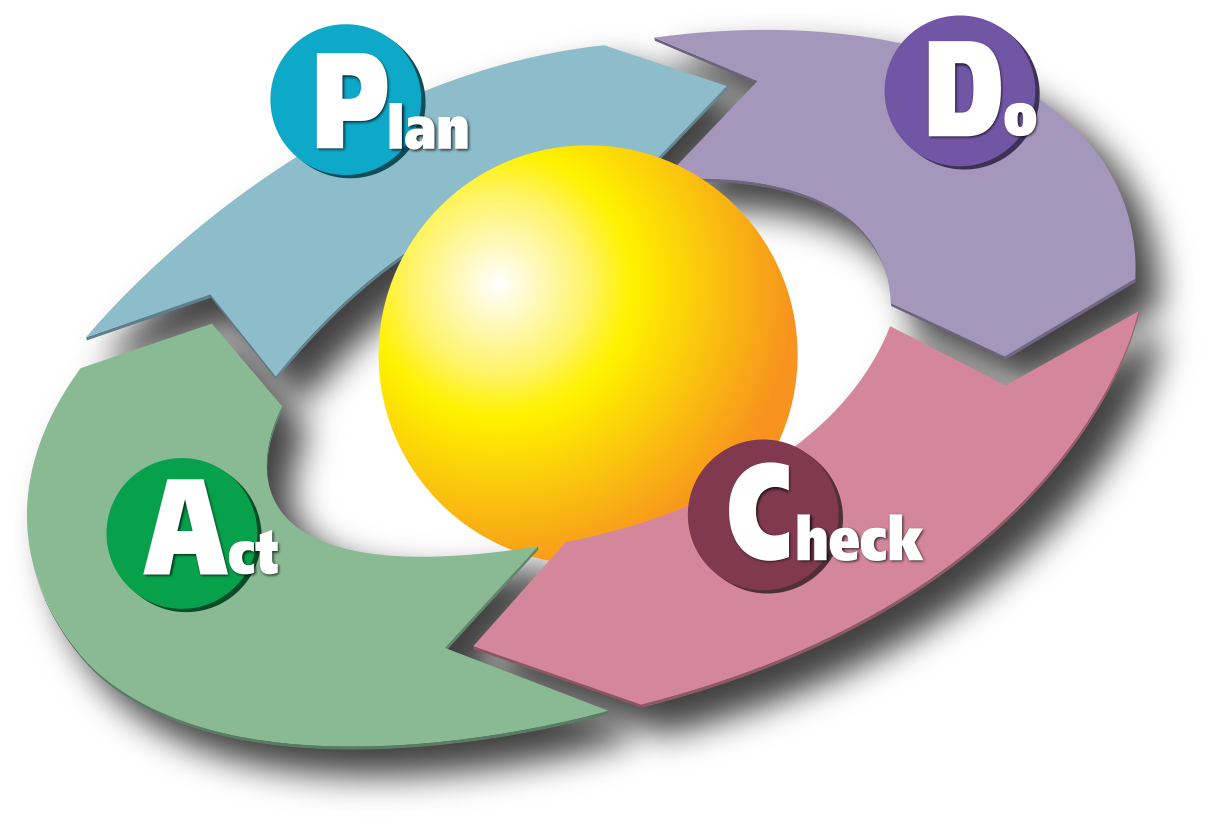
\includegraphics[width=0.5\textwidth, keepaspectratio]{PDCA.png}
    \caption{Ciclo di Deming}
  \end{center}
\end{figure}
\subsection{Standard ISO/IEC 9126}
\label{sec:ISO/IEC9126}
Lo standard \gloss{ISO}/\gloss{IEC} 9126 definisce un modello per migliorare l'organizzazione e i processi, avendo come conseguenza il miglioramento della qualità del prodotto finale. I criteri qualitativi sono divisi in tre macro aree:
\begin{itemize}
  \item{\textbf{Qualità interna:} è la qualità del prodotto software vista dall'interno. Si riferisce alla valutazione del codice sorgente e dell'architettura prima che il prodotto sia ultimato;}
  \item{\textbf{Qualità esterna:} è la qualità del prodotto software vista dall'esterno. Si riferisce al risultato dei test condotti sul prodotto ultimato in un ambiente di prova;}
  \item{\textbf{Qualità in uso:} è la qualità del prodotto vista dall'utilizzatore finale del prodotto. Si riferisce alla qualità dopo il rilascio dell'applicazione.}
\end{itemize}
Non potendo testare la qualità in uso nell'ambito di questo progetto si è scelto di concentrarsi sulla qualità interna ed esterna. Queste qualità nello standard \gloss{ISO}/\gloss{IEC} 9126 sono ulteriormente suddivise in sei categorie:
\begin{figure}[H]
  \begin{center}
    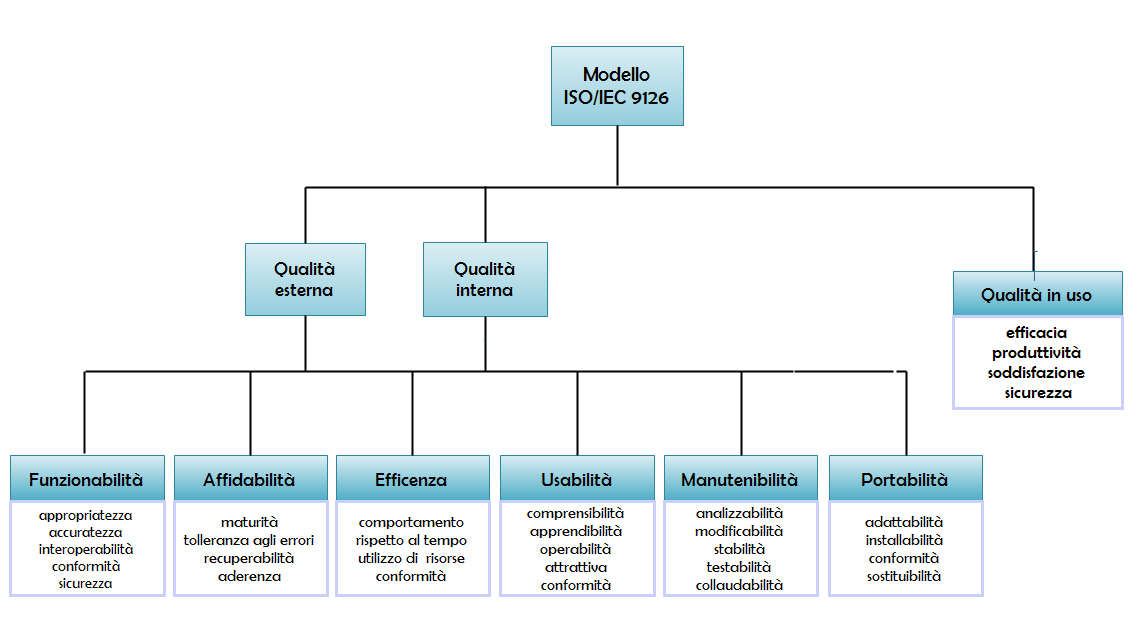
\includegraphics[width=0.9\textwidth, keepaspectratio]{Modello_ISO-IEC_9126.png}
    \caption{Modello dello standard ISO/IEC 9126}
  \end{center}
\end{figure}
\begin{itemize}
  \item{\textbf{Funzionalità:} capacità del prodotto di fornire funzioni che soddisfino esigenze stabilite. Questa categoria si suddivide in:}
    \begin{itemize}
      \item{\textbf{Appropriatezza:} capacità del prodotto di fornire un appropriato insieme di funzioni che rispondano a determinati requisiti;}
      \item{\textbf{Accuratezza:} capacità del prodotto di fornire dei risultati corretti o con precisione concordata;}
      \item{\textbf{Interoperabilità:} capacità del prodotto di interagire con uno o più sistemi esterni;}
      \item{\textbf{Conformità:} capacità del prodotto di aderire a standard del settore di applicazione;}
      \item{\textbf{Sicurezza:} capacità del prodotto di proteggere i dati, ad esempio negando l'accesso a utenti non autorizzati.}
    \end{itemize}
  \item{\textbf{Affidabilità:} capacità del prodotto di mantenere uno specificato livello di prestazioni durante un determinato periodo. Questa categoria si suddivide in:}
    \begin{itemize}
      \item{\textbf{Maturità:} capacità del prodotto di evitare che si verifichino risultati non corretti a causa di errori nel software;}
      \item{\textbf{Tolleranza agli errori:} capacità del prodotto di mantenere uno specificato livello di prestazioni anche in presenza di errori nel software o di uso scorretto del prodotto;}
      \item{\textbf{Recuperabilità:} capacità del prodotto di ristabilire un livello adeguato di prestazioni in seguito a un malfunzionamento;}
      \item{\textbf{Aderenza:} capacità del prodotto di a standard riguardanti l'affidabilità.}
    \end{itemize}
  \item{\textbf{Efficienza:} capacità del prodotto di fornire prestazioni appropriate in relazione alle risorse usate. Questa categoria si suddivide in:}
    \begin{itemize}
      \item{\textbf{Comportamento rispetto al tempo:} capacità del prodotto di fornire i risultati in tempi adeguati;}
      \item{\textbf{Utilizzo delle risorse:} capacità del prodotto di utilizzare le risorse in modo adeguato;}
      \item{\textbf{Conformità:} capacità del prodotto di aderire a standard sull'efficienza.}
    \end{itemize}
  \item{\textbf{Usabilità:} capacità del prodotto di essere capito e usato dall'utente. Questa categoria si suddivide in:}
    \begin{itemize}
      \item{\textbf{Comprensibilità:} facilità di comprensione del prodotto;}
      \item{\textbf{Apprendibilità:} capacità di ridurre l'impegno richiesto all'utente per imparare come usare correttamente il prodotto finale;}
      \item{\textbf{Operabilità:} capacità del prodotto di fare in modo che gli utenti riescano a farne uso per i propri scopi;}
      \item{\textbf{Attrattiva:} capacità del prodotto di essere piacevole per l'utente;}
      \item{\textbf{Conformità:} capacità del prodotto di aderire a standard sull'usabilità.}
    \end{itemize}
  \item{\textbf{Manutenibilità:} capacità del prodotto di essere modificato e migliorato. Questa categoria si suddivide in:}
    \begin{itemize}
      \item{\textbf{Analizzabilità:} facilità di analisi del codice per la localizzazione di errori;}
      \item{\textbf{Modificabilità:} capacità del prodotto di permettere la sostituzione di componenti per implementare una determinata modifica;}
      \item{\textbf{Stabilità:} capacità del prodotto di evitare errori derivanti da modifiche errate;}
      \item{\textbf{Testabilità:} capacità del prodotto di essere facilmente testato rispetto alle modifiche apportate.}
    \end{itemize}
  \item{\textbf{Portabilità:} capacità del prodotto di essere trasportato in un altro ambiente di lavoro. Questa categoria si suddivide in:}
    \begin{itemize}
      \item{\textbf{Adattabilità:} capacità del prodotto di essere adattato per ambienti operativi diversi senza modifiche diverse da quelle fornite;}
      \item{\textbf{Installabilità:} capacità del prodotto di essere installato in specifici ambienti;}
      \item{\textbf{Conformità:} capacità del prodotto di aderire a standard sulla portabilità;}
      \item{\textbf{Sostituibilità:} capacità del prodotto di essere utilizzato al posto di un altro software per svolgere gli stessi compiti.}
    \end{itemize}
\end{itemize}
\newpage
\section{Resoconto attività di verifica}
\label{sec:resAttivitaVerifica}
\subsection{Documenti}
Nella tabella di seguito sono riportati i valori degli indici di Gulpease per ogni documento prodotto durante l'attività di Analisi. L'esito della verifica dipenderà dal valore di questo indice come descritto nella sezione \ref{par:metricheGulpease}.
\begin{center}
  \begin{tabular}{| c | c | c |}
    \hline
    Documento & Valore indice & Esito\\
    \hline
    \textit{Studio di Fattibilità v1.0.0} & 54.18 & Superato\\
    \textit{Norme di Progetto v1.0.0} & 52.04 & Superato\\
    \textit{Piano di Progetto v1.0.0} & 54.87 & Superato\\
    \textit{Piano di Qualifica v1.0.0} & 52.82 & Superato\\
    \textit{Analisi dei Requisiti v1.0.0} & 68.06 & Superato\\
    \textit{Glossario v1.0.0} & 47.42 & Superato\\
    \hline
  \end{tabular}
\end{center}
\newpage
\section{Pianificazione dei test}
Di seguito sono descritti i test di sistema. In futuro questa sezione verrà aggiornata con i test di integrazione e di unità.
\subsection{Test di sistema}
I test di sistema permettono di verificare il comportamento del sistema rispetto ai requisiti descritti nell'\href{run:./AnalisiDeiRequisiti\_v1.0.0.pdf}{Analisi dei requisiti v1.0.0}.\\
La tabella seguente descrive i test dei requisiti ritenuti meritevoli di verifica. \\
La colonna "Stato" nella tabella è lasciata vuota in quanto i test saranno effettuati successivamente.
%TODO completare tabella bella
\begin{center}
  \begin{tabular}{| c | l | l | c |}
    \hline
    Test & Descrizione & Stato & Requisito\\
    \hline
    Tcodreq & descreq &  & codreq\\
    \hline
  \end{tabular}
\end{center}
\end{document}